% tk_test_pyramid: testing pyramid, three layers in neutral greys (DIAGRAMS.md item 19)
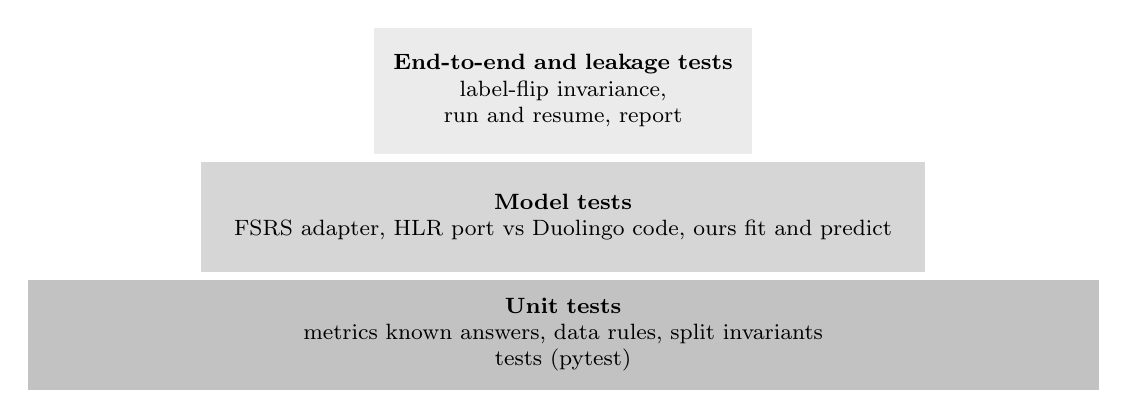
\begin{tikzpicture}[font=\footnotesize]
  \fill[black!8] (-2.4,3.0) rectangle (2.4,4.6);
  \fill[black!16] (-4.6,1.5) rectangle (4.6,2.9);
  \fill[black!24] (-6.8,0.0) rectangle (6.8,1.4);
  \node[align=center, text width=4.6cm] at (0,3.8)
    {\textbf{End-to-end and leakage tests}\\label-flip invariance, run and resume, report};
  \node[align=center, text width=8.8cm] at (0,2.2)
    {\textbf{Model tests}\\FSRS adapter, HLR port vs Duolingo code, ours fit and predict};
  \node[align=center, text width=12.8cm] at (0,0.7)
    {\textbf{Unit tests}\\metrics known answers, data rules, split invariants\\\NumBenchTests{} tests (pytest)};
\end{tikzpicture}
